\chapter{Background}

\section{Hardware}
\subsection{Particle Photon}
Particle Photon is a tiny board (36.58mm $\times$ 20.32mm $\times$ 4.32mm in our configuration, weighing in at 5 grams) specifically designed for Internet of Things (IoT)\footnote{A system of typically embedded devices that connects to the Internet and to each other, without requiring human-to-human or human-to-computer interaction \cite{WikipediaIoT}. There's still no baseline or standard definition, which is why IEEE is asking for suggestions to the community to provide it \cite{IEEEIoT}.} projects \cite{ParticlePhoton}, based on a relatively powerful but power efficient microcontroller of the STM32 ARM Cortex M3 family, with integrated Wi-Fi and the ability to interface itself with cloud services offered by Particle.

Unfortunately, the integrated Wi-Fi module has not been powerful enough to ensure a reliable connection in the tested scenarios, causing frequent disconnections. An Airgain's IPEX antenna, easily pluggable to the Photon through a U.FL connector, has allowed to achieve a more stable connection.
The code deployment can be performed seamlessly through a web-based IDE, that compiles and flashes the code to the selected device Over-The-Air (OTA). It is also possible to control the real-time device's status through a web-based console, that allows to flash the firmware to a specific version (downgrades are trickier than upgrades, especially OTA), and displays graphs for data such Wi-Fi's signal strength and quality, round trip time and memory usage.

\begin{center}
	\begin{figure}[ht]
		\makebox[\textwidth]{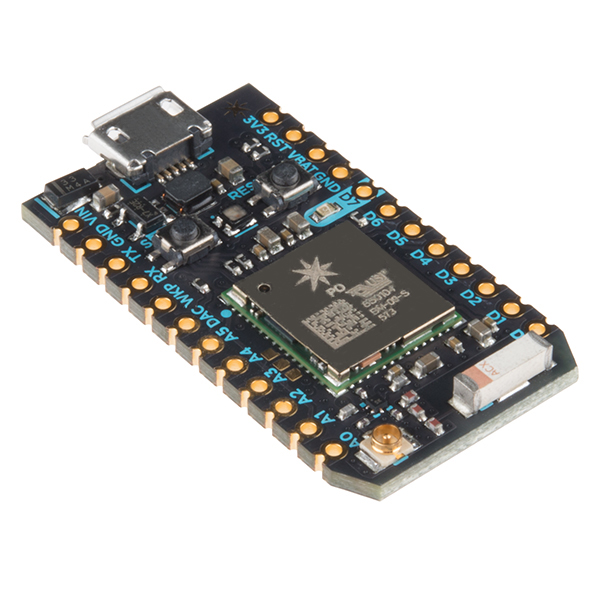
\includegraphics[width=0.3\paperwidth]{img/photon.jpg}}
		\caption{Particle Photon \cite{Photon}.}
	\end{figure}
\end{center}

\subsection{Sensors}
The SparkFun's sensor stick used in the project is a 9 Degrees of Freedom (9DoF) Magnetic, Angular Rate and Gravity (MARG) Micro-Electro-Mechanical Systems (MEMS) sensor. Its inertial module is the STMicroelectronics's LSM9DS1 integrated circuit, that features a digital linear acceleration sensor, a digital angular rate sensor and a digital magnetic sensor: each one can take measurements from $x$, $y$ and $z$ axes, and that's where the 9 degrees of freedom come from.

The stick has been connected to the Photon through the I$^2$C serial bus interface. Its compact size and power efficiency make it ideal for embedded systems \cite{SensorDatasheet}.

\begin{center}
	\begin{figure}[ht]
		\makebox[\textwidth]{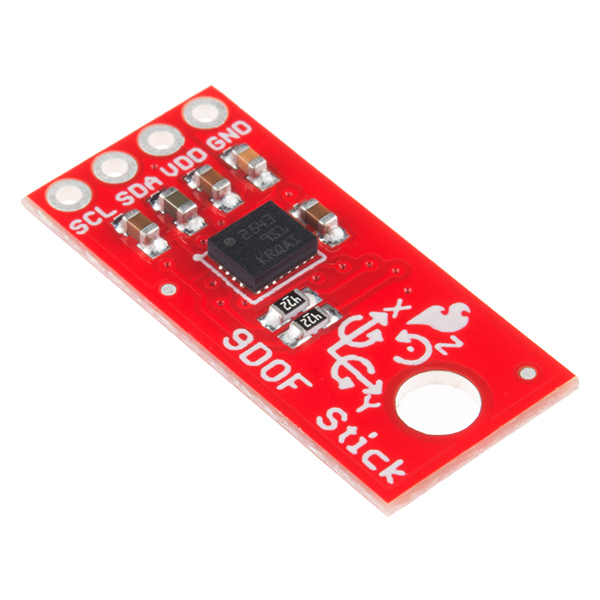
\includegraphics[width=0.3\paperwidth]{img/imu.jpg}}
		\caption{SparkFun Sensor Stick \cite{IMU}.}
	\end{figure}
\end{center}

\section{Software}

\subsection{Node.js}
Node.js is an open-source asynchronous event-driven JavaScript runtime environment that executes code outside of a browser, built on Google Chrome's V8 JavaScript engine \cite{Node.js}.

To put it simply, a synchronous execution environment needs to wait to one task to finish before moving to another; asynchronous execution, on the contrary, allows to move to another task before the previous one has finished. In a typically input/output (I/O) bound context, (like the network), for a single-threaded software (like Node.js) an asynchronous (non-blocking) I/O method allows to register the clients' requests, wait until the reply is available, and then call the related callback. This allows faster replies to the clients, compared to synchronous (blocking) I/O.

\subsection{Express.js}
Express.js, or simply Express, is a minimalist, open-source web framework for Node.js, designed for building web applications and APIs \cite{Express.js}. Its main feature is the routing mechanism: it allows to specify a callback function called when the application receives a request to the specified route and HTTP method. For example, using an Express \texttt{app} object, \texttt{app.get()} would handle GET requests, \texttt{app.post()} would handle POST ones, and so on.

\subsection{Three.js}
Three.js is a JavaScript library for creating animated 3D graphics in a web browser. Three.js uses WebGL (and simplifies its API) for creating GPU-accelerated 3D animations within web browsers without relying on proprietary plugins; in fact, Three.js is fully open-source.

\subsection{MQTT}
Message Queue Telemetry Transport (MQTT) is a machine-to-machine (M2M)/IoT connectivity protocol \cite{MQTT}. MQTT was designed as an extremely lightweight publish/subscribe messaging transport, and can be supported by any network protocol that provides ordered, lossless and bi-directional connections (typically TCP/IP) \cite{MQTTDoc}.

The MQTT protocol defines two types of network entities: a message broker (Mosca in the project) and a number of clients. An MQTT broker is a server that receives all messages from the clients and then routes the messages to the appropriate destination clients \cite{KnowMQTT}. An MQTT client is any device that runs an MQTT library and connects to an MQTT broker over a network \cite{ClientBroker}.

Information is organized in a hierarchy of topics. When a publisher has a new item of data to distribute, it sends a control message with the data to the connected broker. The broker then distributes the information to any clients that have subscribed to that topic. The publisher does not need to have any data on the number or locations of subscribers, and subscribers in turn do not have to be configured with any data about the publishers.

\subsection{MongoDB}
MongoDB is a general purpose, document-based, distributed database \cite{MongoDB}. Classified as a NoSQL database, it stores documents in a JSON-like format. MongoDB belongs to the category of document-oriented databases: the smallest unit of storage is a document; documents are stored in collections, which in turn make up a database. Documents are analogous to rows in a SQL table, but with one big difference: documents may have different structures. Another feature of MongoDB is that fields in a document can contain arrays and or sub-documents (sometimes called nested or embedded documents).

MongoDB stores data records as BSON documents. BSON is a binary representation of JSON documents, although it contains more data types than JSON \cite{BSONSpec}.

\subsection{TensorFlow}
\dots

\section{Rotation formalisms}
This section describes the mathematical formalisms to represent three-dimensional rotations in the project.

\subsection{Tait–Bryan angles}
Tait–Bryan angles (also called nautical angles or \textit{yaw, pitch and roll}) are a variant of Euler angles, normally used for aerospace applications (wherein they are often called Euler angles). Euler angles are a minimal representation (a set of three numbers) of relative orientation. This set of three angles describes a sequence of rotations about the axes of a reference frame. There are, however, sets that describe the same orientation: different combinations of $x$, $y$, and $z$ axes lead to different Euler angles \cite{Rob20}.

The only difference is that Tait–Bryan angles represent rotations about three distinct axes (e.g. $x$-$y$-$z$), while proper Euler angles use the same axis for both the first and third elemental rotations (e.g. $z$-$x$-$z$) \cite{WikipediaEulerAngles}.

Once fixed a reference frame, \textit{yaw, pitch and roll} represent the rotation angle around the $z$, $y$, and $x$ axis, respectively.
If the rotation occurs about the axes of the original coordinate system, which remains motionless, the rotation is called \textit{extrinsic}, and when it occurs about the axes of the rotating coordinate system, which changes its orientation after each elemental rotation, the rotation is called \textit{intrinsic}. It's interesting to know that $z$-$y$-$x$ intrinsic rotations correspond to $x$-$y$-$z$ extrinsic ones, and the same applies to every reversed-order rotation.

\begin{center}
	\begin{figure}[ht]
		\makebox[\textwidth]{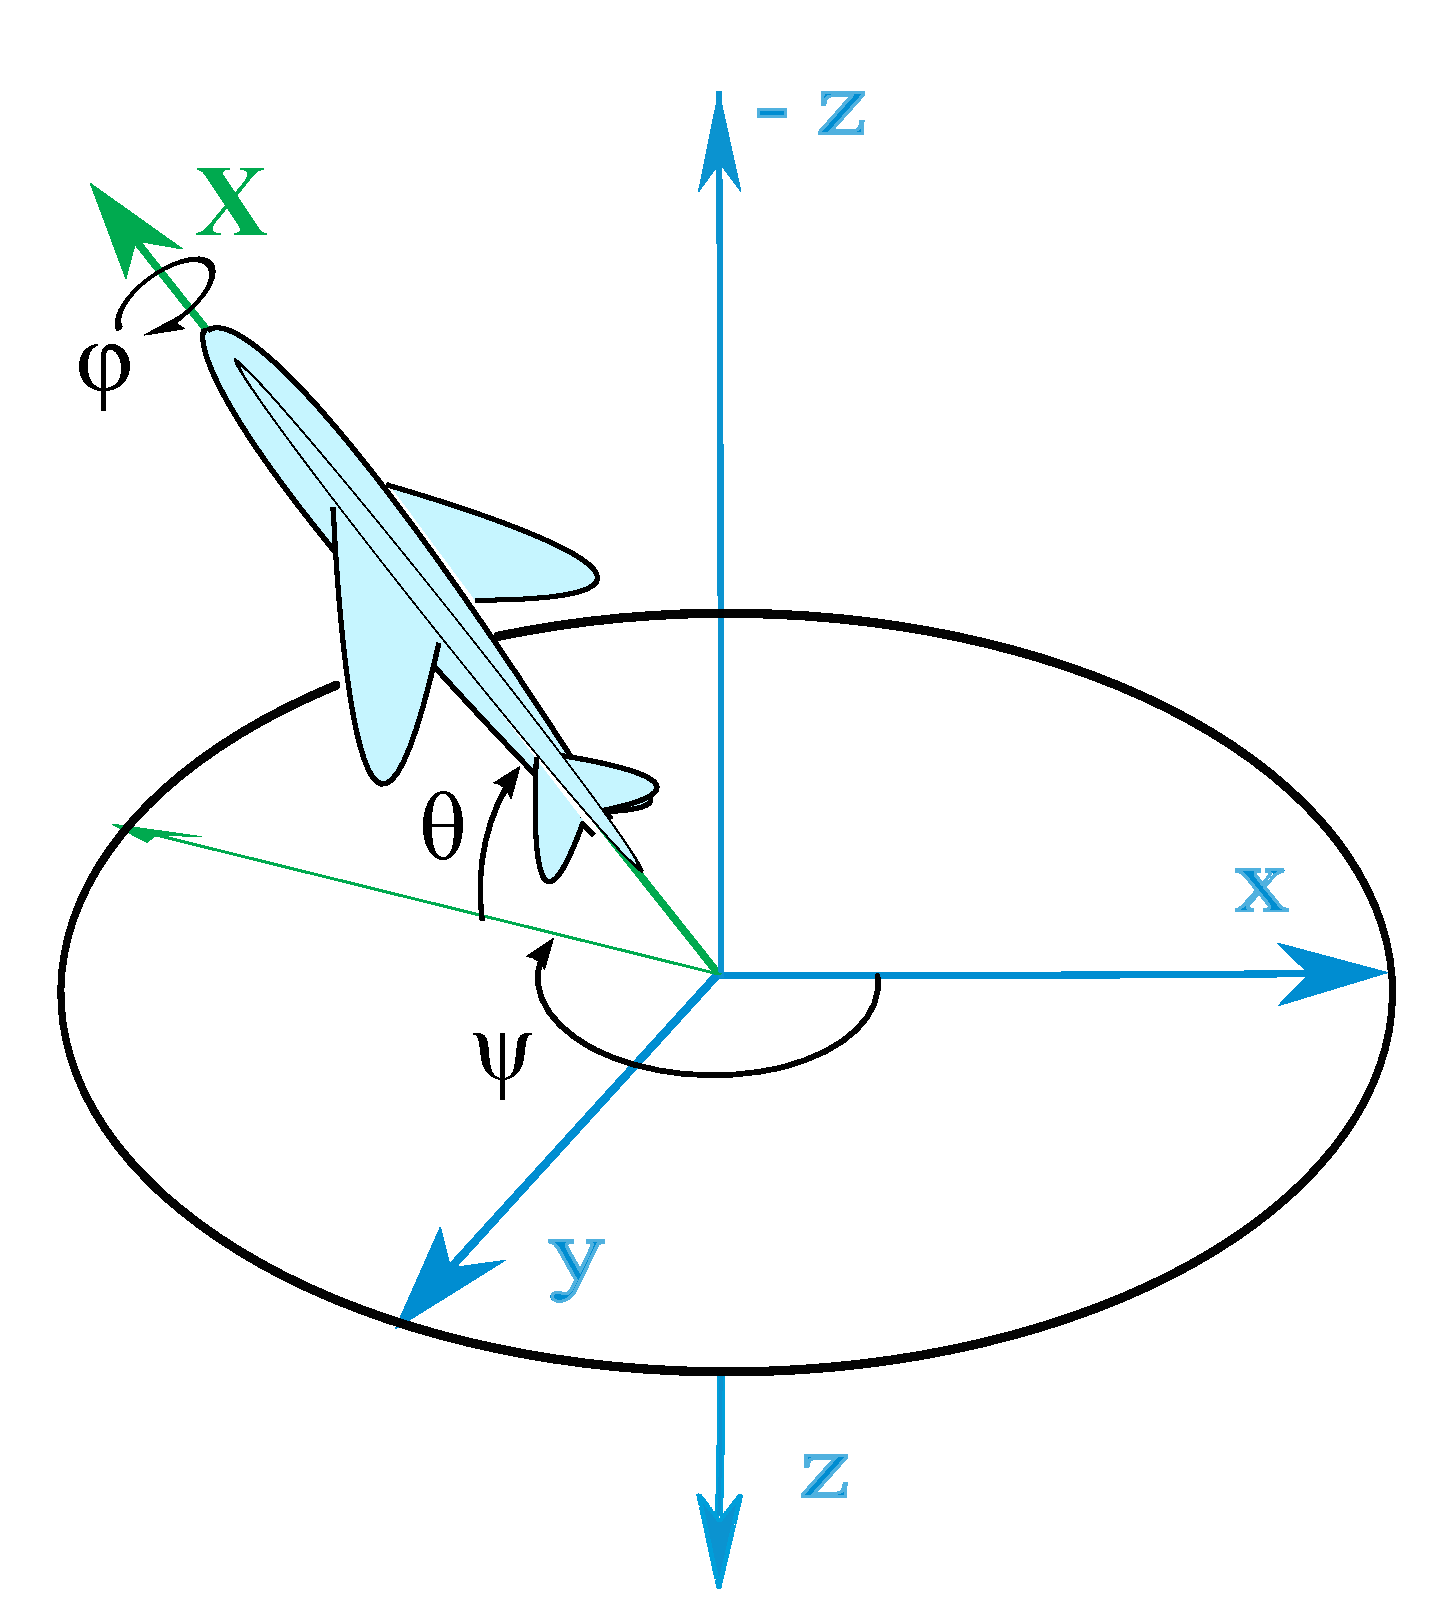
\includegraphics[width=0.35\paperwidth]{img/plane.pdf}}
		\caption{Yaw ($\psi$), pitch ($\theta$) and roll ($\varphi$) angles for an aircraft \cite{WikimediaPlane}.}
	\end{figure}
\end{center}
Representations with Euler angles share a problem called \textit{gimbal}\footnote{A \textit{gimbal} is a pivoted support that allows the rotation of an object about a single axis.} \textit{lock}\footnote{The word lock is misleading: no gimbal is restrained.}, that occurs when the orientation of the sensor cannot be uniquely represented, and causes a loss of a degree of freedom \cite{Dil18}.

An example: when the device pitches up 90$^{\circ}$ its pitch and yaw gimbals become aligned, and changes to roll and yaw apply the same rotation to the device \cite[68]{Tit04}.

This is a well-known problem for animating rotations, and it can be solved by adding a fourth gimbal actively driven by a motor so as to maintain a large angle between roll and yaw gimbal axes \cite{Bie99}, by mounting the inertial sensors directly to the body of the device (\textit{strapdown systems}) \cite[3]{Tit04}, or by representing rotations using quaternions instead of Euler angles.

\subsection{Quaternions}
Quaternions\footnote{Invented in 1843 by the famous mathematical physicist William Rowan Hamilton, they had been already described by Gauss in 1819, but his work was not published until 1900 \cite{Puj12}.} are four-dimensional entities that extend the complex numbers, and represent elements of $\mathbb{R}^4$ \cite{Ham47}. Compared to Euler angles, they are simpler to compose and avoid the problem of gimbal lock. Compared to rotation matrices, they are more compact, more numerically stable, and more efficient (more than twice as efficient as matrices on memory, and the quaternion multiplication is more than 1.5 times faster than matrix multiplication \cite{Gol10}).

As it represents an element of $\mathbb{R}^4$, a quaternion can be written as:

\begin{center}
	$q = (q_0, q_1, q_2, q_3)$
\end{center}
where $q_0$, $q_1$, $q_2$, and $q_3$ are real numbers, but it is generally represented this way:

\begin{center}
	$\textbf{q} = q_0 + \textbf{i}q_1 + \textbf{j}q_2 + \textbf{k}q_3$
\end{center}
where \textbf{i}, \textbf{j} and \textbf{k} are the standard orthonormal basis in $\mathbb{R}^3$ \cite{Kui99}; it always follows the fundamental formula of quaternion algebra:

\begin{center}
	$\textbf{i}^2 = \textbf{j}^2 = \textbf{k}^2 = \textbf{ijk} = -1$
\end{center}
Quaternions have a fundamental role in the project, since the Madgwick filter \cite{Mad10} and the 3D representation through Three.js heavily rely on them.

Algebra behind quaternions rotations will not be treated, because its complexity doesn't allow to simplify the main concepts in few lines; however, it can be found in \cite[127-134]{Kui99}.

\subsection{Rotation matrix}
In two dimensions, a rotation matrix $R \in \mathbb R^{2 \times 2}$ is a matrix that is used to perform a rotation in Euclidean space. Given a vector $\vec u \in \mathbb R^2$ and an angle $\theta \in \mathbb R$, the vector $\vec u$ rotated through an angle $\theta$ can be written as $R(\theta) \vec u$.

The matrix

\[
	R =
	{\begin{pmatrix}
		\cos \theta & -\sin \theta \\
		\sin \theta & \cos \theta
	\end{pmatrix}}
\]
rotates points in the $xy$-plane counterclockwise in a \textit{right-handed coordinate system} ($y$ counterclockwise from $x$) through an angle $\theta$ with respect to the $x$ axis about the origin of a two-dimensional Cartesian coordinate system. To perform the rotation of a point $p$ with coordinates ($x$, $y$), it should be written as column vector, and multiplied by the matrix $R$:

\[
	p_{rotated} = Rp =
	{\begin{pmatrix}
		\cos \theta &-\sin \theta \\
		\sin \theta &\cos \theta
	\end{pmatrix}}
	\cdot
	{\begin{pmatrix}
		x \\
		y
	\end{pmatrix}} =
	{\begin{pmatrix}
		x\cos \theta -y\sin \theta \\
		x\sin \theta +y\cos \theta
	\end{pmatrix}}
\]
How to represent \textit{yaw, pitch and roll}?\\
A \textit{yaw} is a counterclockwise (CCW) rotation of $\alpha$ on the $z$-axis. The rotation matrix is
\[
	R_z(\alpha) =
	\begin{pmatrix}
		\cos\alpha & -\sin\alpha & 0 \\
		\sin\alpha & \cos\alpha & 0 \\
		0 & 0 & 1
	\end{pmatrix}
\]
Note that the upper left values compose a 2D rotation matrix, and the coordinates on the third dimension (around whom the rotation happens) are left unchanged. The same applies to the other two matrices, but with the second and the first dimension.\\
A \textit{pitch} is a CCW rotation of $\beta$ on the $y$-axis. The rotation matrix is
\[
	R_y(\beta) =
	\begin{pmatrix}
		\cos\beta & 0 & \sin\beta \\
		0 & 1 & 0 \\
		-sin\beta & 0 & \cos\beta
	\end{pmatrix}
\]
A \textit{roll} is a CCW rotation of $\gamma$ on the $x$-axis. The rotation matrix is
\[
	R_x(\gamma) =
	\begin{pmatrix}
		1 & 0 & 0 \\
		0 & \cos\gamma & -\sin\gamma \\
		0 & sin\gamma & \cos\gamma
	\end{pmatrix}
\]
The final rotation matrix is obtained by the multiplication of the previous three:
\begin{gather*}
	R(\alpha, \beta, \gamma) = R_z(\alpha) R_y(\beta) R_x(\gamma) = \\
	\begin{pmatrix}
		\cos\alpha \cos\beta & \cos\alpha \sin\beta \sin\gamma - \sin\alpha \cos\gamma & \cos\alpha \sin\beta \cos\gamma + \sin\alpha \sin\gamma \\
		\sin\alpha \cos\beta & \sin\alpha \sin\beta \sin\gamma + \cos\alpha \cos\gamma & \sin\alpha \sin\beta \cos\gamma - \cos\alpha \sin\gamma \\
		-\sin\beta & \cos\beta \sin\gamma & \cos\beta \cos\gamma
	\end{pmatrix}
\end{gather*}
It is important to note that $R(\alpha, \beta, \gamma)$ performs the roll first, then the pitch, and finally the yaw. If the order of these operations is changed, a different rotation matrix results \cite{Lav06}.

Given an acceleration vector $\vec a$, the rotated one is obtained by the matrix-vector multiplication

\[
	\vec a_r = R(\alpha, \beta, \gamma) \vec a
\]

\subsection{Spherical coordinates}
Spherical coordinates specify the position of a point in a three-dimensional space using three numbers: $\rho$, $\theta$ and $\phi$, where $\rho$ represents the radial distance of the point from the origin, $\theta$ represents the angle of the the $z$-axis with the line that represents the distance, and $\phi$ represents the angle between the $x$-axis and the projection of the point on the plane generated by the $xy$-axes \cite{Sok}.

\begin{center}
	\begin{figure}[ht]
		\makebox[\textwidth]{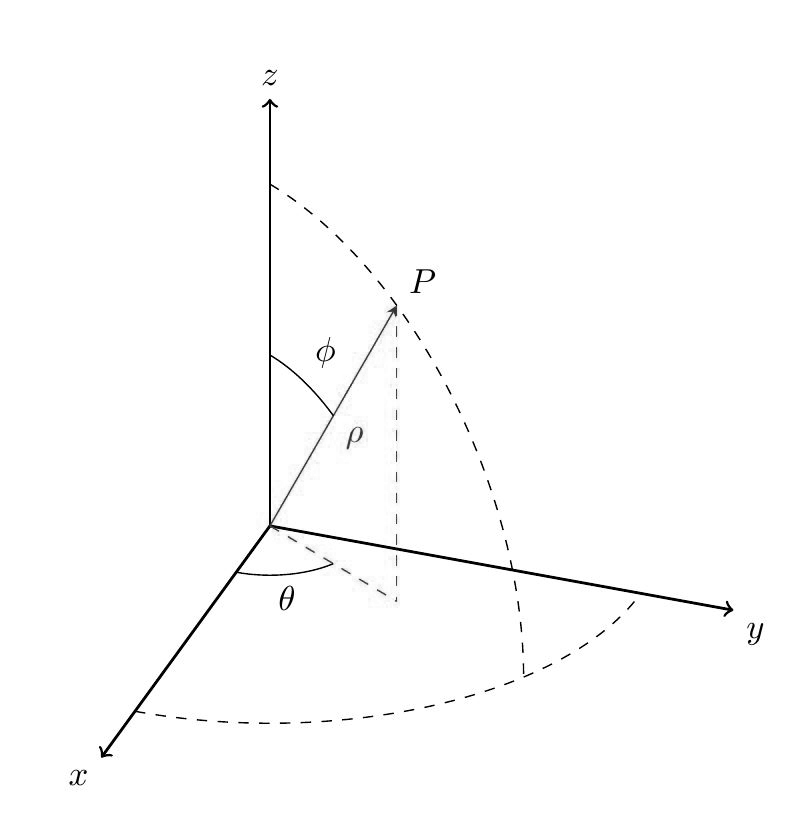
\includegraphics[width=0.45\paperwidth]{img/spherical_acc.jpg}}
		\caption{Spherical coordinates of the point P \cite{HartleySpherical}.}
	\end{figure}
\end{center}
The spherical coordinates are related to the Cartesian ones ($x$, $y$ and $z$) by the formulas \cite{Sok}

\[
	x = \rho \cos\phi \sin\theta \quad\quad y = \rho \sin\phi \sin\theta \quad\quad  z = \rho \cos\theta
\]
where the typical constraints

\[
	0 \leq \rho < \infty \quad\quad 0 \leq \phi < 2\pi \quad\quad 0 \leq \theta \leq \pi
\]
ensure an unique representation.

\section{Filters}
Motion representation can be obtained through accelerometer reading within the $x$, $y$ and $z$ axes, that make up an acceleration vector.

MEMS sensors are known to be very noisy, especially when working at high reading frequencies \cite[7]{Mat08}, and the noise is of a specific type, the Additive White\footnote{White noise is a random signal with constant amplitude across the whole frequency spectrum.} Gaussian\footnote{Noise with a probability density function equal to that of the normal distribution, which is also known as the Gaussian distribution \cite{WikipediaGaussianNoise}.} Noise (AWGN) \cite{Yas03}. An effective way to remove AWGN is to use the Kalman filter \cite{Ko07, Sär15}, as it assumes that the errors are Gaussian \cite{Kal60}.

\subsection{Kalman filter}
Kalman filtering, also known as linear quadratic estimation (LQE) \cite{Ma19}, is an efficient recursive algorithm that uses a series of measurements observed over time, containing statistical noise and other inaccuracies, and produces estimates of unknown variables (the internal state of a linear dynamic system\footnote{Linear dynamic systems are systems in which its evolution is described by a linear function and hence satisfies the superposition principle.} \cite[47]{Ma19}) \cite[7-8]{Ma19}. This approach tends to be more precise than those based on a single measurement alone, because it uses using Bayesian inference and estimates a joint probability distribution over the variables for each timeframe \cite[8]{Ma19}.

Kalman filter is most often conceptualized as two distinct phases \cite[12-13]{Ma19}:

\begin{itemize}
	\item time updating: prediction phase, where the previous timesteps are used to predict the current one's state (\textit{a priori} state estimate);
	\item measure update: observation phase, where the prediction is combined with the current observation information to refine the state estimate (\textit{a posteriori} state estimate).
\end{itemize}

The Kalman filter has numerous applications in technology, like navigation and control of vehicles, particularly aircraft, spacecraft and dynamically positioned ships \cite{WikipediaKalman}.

\subsection{Madgwick filter} \label{Madgwick filter}
In 2009 Sebastian O. H. Madgwick, as part of his Ph.D research at the University of Bristol, developed an orientation filter for IMU (6DoF: tri-axis gyroscope and accelerometer) and MARG (9DoF: IMU + tri-axis magnetometer) sensors.

The filter is based on an optimized gradient-descent algorithm that fuses together the \textit{raw} data from the sensors \cite{Mad10}, and uses an analytically derived Jacobian matrix\footnote{A matrix of partial derivatives of a function.} to find a quaternion that minimizes the estimation's error \cite{Che12}.
\bigbreak

There are three interesting features \cite{Mad10}:
\begin{itemize}
	\item it is computationally inexpensive, thanks to the quaternion representation of rotation;
	\item it is effective at relatively low sampling rates, e.g. 10 Hertz. This is a big advantage, because Kalman-based filters may require sampling rates that exceed the bandwidth;
	\item its parameters can be changed according to the usage environment characteristics.
\end{itemize}

The low computational load reduces the hardware and power necessary for inertial movement tracking, allowing to create lightweight and inexpensive systems, capable of functioning for extended periods of time \cite{Mad11}.

\section{Neural networks}
Machine learning is a subfield of computer science that studies algorithms and statistical models to construct computer programs that automatically improve with experience \cite{Mit97}. Machines don't really learn\footnote{The name ``machine learning" was coined by Arthur Samuel in 1959, while working for IBM on computers that learned how to play checkers when given only the rules of the game \cite{Sam59}.}, but typically build a mathematical function that produces the desired output when applied to a collection of inputs, called \textit{training data}, and this function is used to make predictions on inputs not encountered during training. The ability to make accurate predictions on new data is called \textit{generalization} \cite{Hay08}.
\bigbreak

There are two kinds of ``learning'' processes:
\begin{itemize}
	\item \textit{supervised}, when the training data is labeled or classified with the correct answer, and the network can use it to improve its performance. The goal is to minimize a loss function, which quantifies the training error; the networks are most often trained with the \textit{backpropagation}, a gradient-descent algorithm that computes the gradient of the loss function, to change them accordingly to the training;
	\item \textit{unsupervised}, when the training data is neither labeled or classified, and the network has to find by itself the way to categorize the data. In this case, the performance measurement is task-independent \cite{Hay08}.
\end{itemize}
One of the most famous statistical model for machine learning is the artificial neural network, commonly referred as ``neural network''. It's composed of multiple layers of inter-connected nodes. The term \textit{neural} suggest the parallelism with the biological neural networks that form animal brains, since the Rosenblatt's \textit{perceptron}\footnote{After the McCulloch and Pitt’s neuron, the perceptron was the next step towards the neural networks.} was born to mimic certain part of the neuron, such as dendrites, that receive the electrochemical stimulation from other neural cells, and axons, that propagates it.

The building block of the neural networks is the \textit{neuron}, an information-processing unit that works in this way: takes the inputs from weighted links, adds the weighted input signals together, and finally uses the sum as an input for the activation function; this function's output can be an input for another neuron, or part of the network's output.

\begin{center}
	\begin{figure}[ht]
		\makebox[\textwidth]{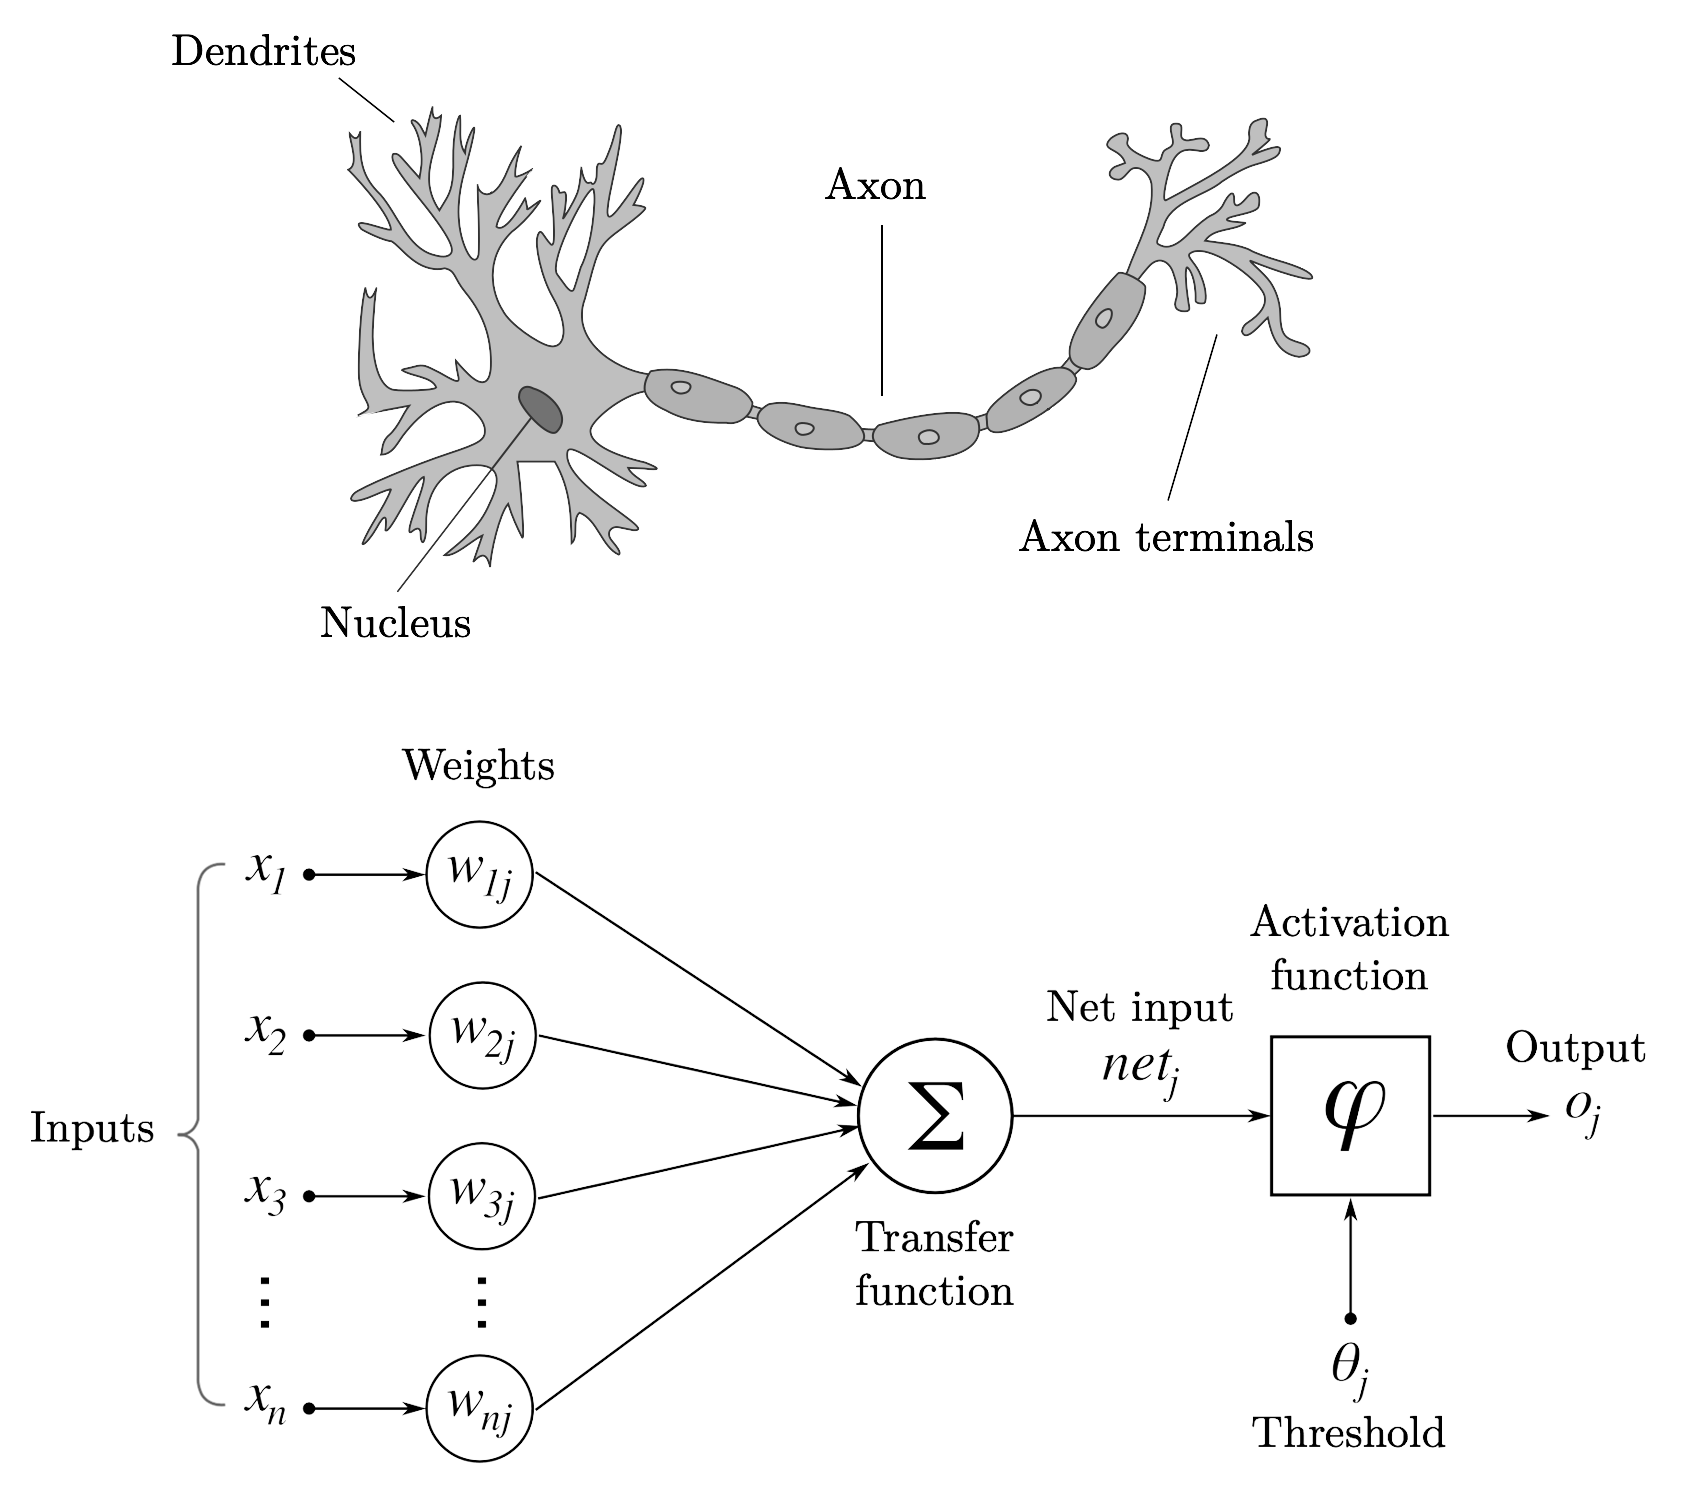
\includegraphics[width=0.65\paperwidth]{img/artificial_biological_network.png}}
		\caption{Similarities between biological \cite{WikipediaNeuron} and artificial neurons.}
	\end{figure}
\end{center}
There are three fundamentally different classes of network architectures \cite{Hay08}:

\begin{itemize}
	\item \textbf{single-layer feedforward networks}: in a layered network, the neurons are organized in form of layers, and in this case, the first layer of nodes, also called \textit{input layer}, feeds its output directly to the last (second) layer, called \textit{output layer}, where the neurons perform the computation. These networks are called \textit{feedforward} because the information moves in only one direction, forward, from the input nodes to the output ones;
	\item \textbf{multi-layer feedforward networks}: in this model, between the input and the output layer, there are one or more \textit{hidden layers} of neurons. The term ``hidden'' refers to the fact they're not seen directly from either the input or output of the network. By adding hidden layers, the network is capable to extract higher-order statistics from its input;
	\item \textbf{recurrent networks}: differently from feedforward neural networks, in this architecture there is at least one feedback loop. Feedforward neural network remember what they learnt during training, while recurrent ones, in addition, remember things learnt from previous inputs while generating outputs. Along with the fact that this model can deal with variable length inputs, makes them applicable to time-dependent tasks, like weather forecasting or speech recognition.
\end{itemize}

\begin{center}
	\begin{figure}[ht]
		\makebox[\textwidth]{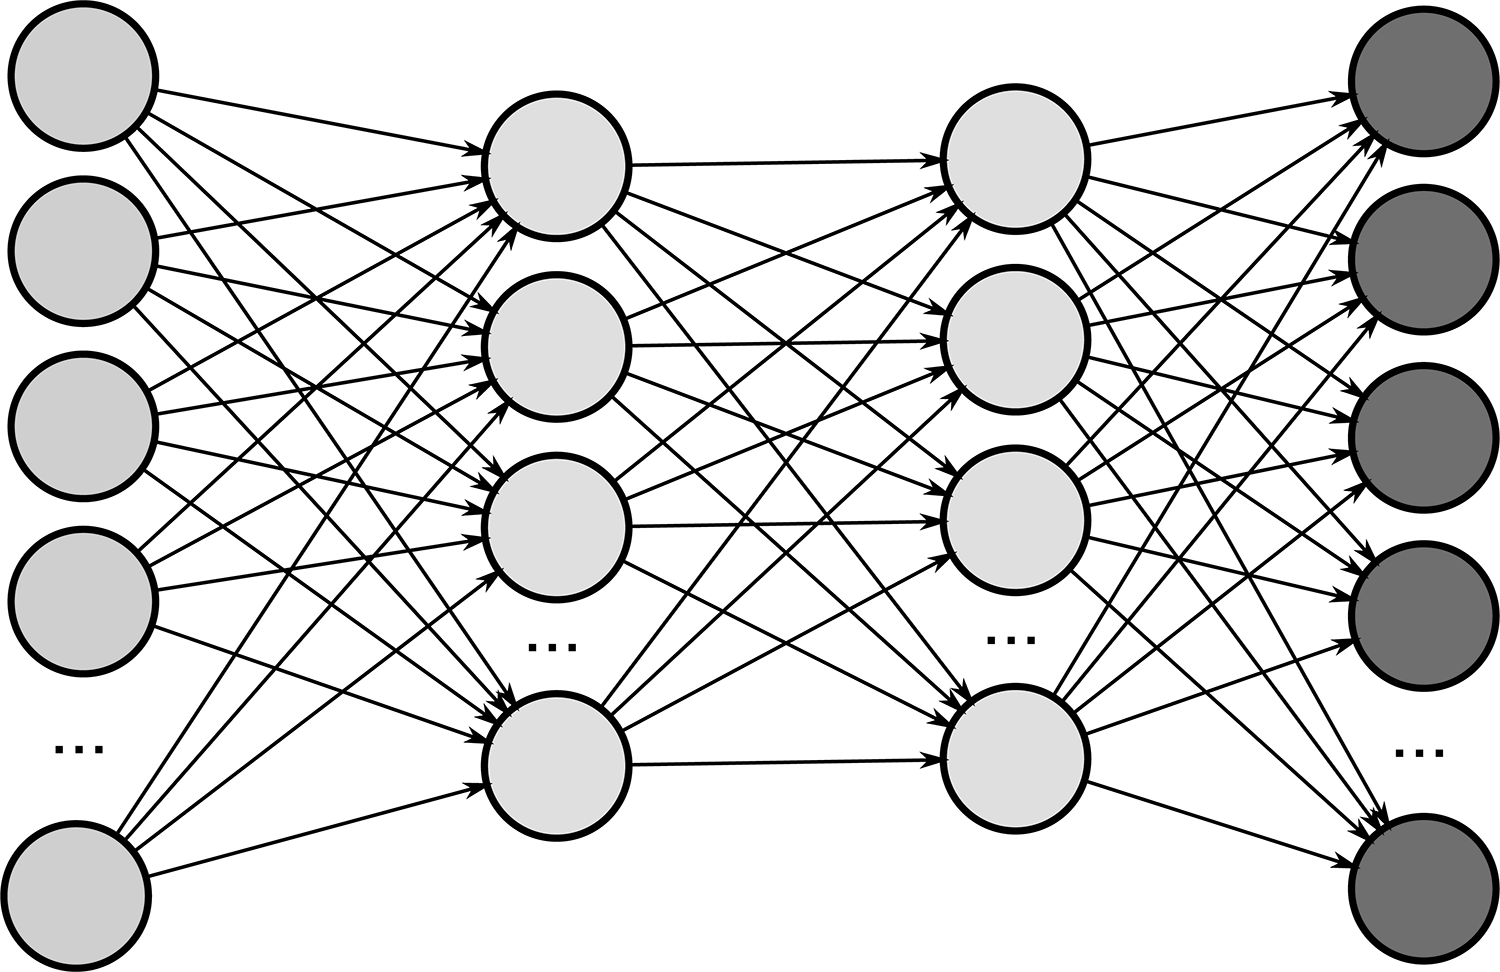
\includegraphics[width=0.4\paperwidth]{img/neural_network.png}}
		\caption{A fully-connected feedforward neural network with two hidden layers.}
	\end{figure}
\end{center}

\subsection{Time delay neural networks}
Time delay neural network (TDNN) is one of the simplest neural network that provides \textit{shift-invariant} pattern classification. \textit{Shift-invariance} means that different displacements of the features in the pattern don't affect the prediction. TDNNs were invented in 1989 to classify phonemes in speech signals for automatic speech recognition; the fact that the TDNN recognizes phonemes independently of their position in time, significantly improved the performance over static classification \cite{Wai89}.
\bigbreak

TDNNs are most often implemented by the machine learning frameworks with 1-dimensional convolutional neural network (CNN).\\
2-dimensional CNNs are widely used for image classification, where the two dimensions are the $x$ and the $y$ axis; in time series classification, of course, the only dimension is the time.
\bigbreak

Convolution is a linear mathematical operator defined as the integral of the product of two functions, that produces a third function; CNNs use convolution in place of general matrix multiplication \cite{Goo16}. The convolution is defined as:

\[
	(f*g)(t)\,
		\triangleq
	\int_{-\infty }^{\infty} f(\tau)g(t-\tau)\, d\tau\,
		=
	\int_{-\infty }^{\infty} f(t-\tau)g(\tau)\, d\tau
\]
\newline
In CNNs, there are two types of layers:
\begin{itemize}
	\item the \textit{convolutional layer}, that through a fixed-size window, called \textit{kernel}, slides over the inputs and gives its outputs to the next layer. The kernel of \textit{filters} computes the dot product between its weights and the inputs (this process is called \textit{convolution}), and projects the output in a n-dimensional space, where n is the number of output filters in the convolution;
	\item the \textit{pooling layer}, that takes the maximum value of the input's patch (max-pooling) or the average (average-pooling), or other values by using different approaches, performing a down-sampling.
\end{itemize} 
The \textit{shift-invariance} is provided by the kernel's \textit{weights sharing}, that means that the same weights are used across the entire layer's input, so they will learn independently of their position. The kernel's shift over the input after every step is called \textit{stride}, and it's typically 1, but it can be higher to perform down-sampling.
\bigbreak

\begin{center}
	\begin{figure}[ht]
		\makebox[\textwidth]{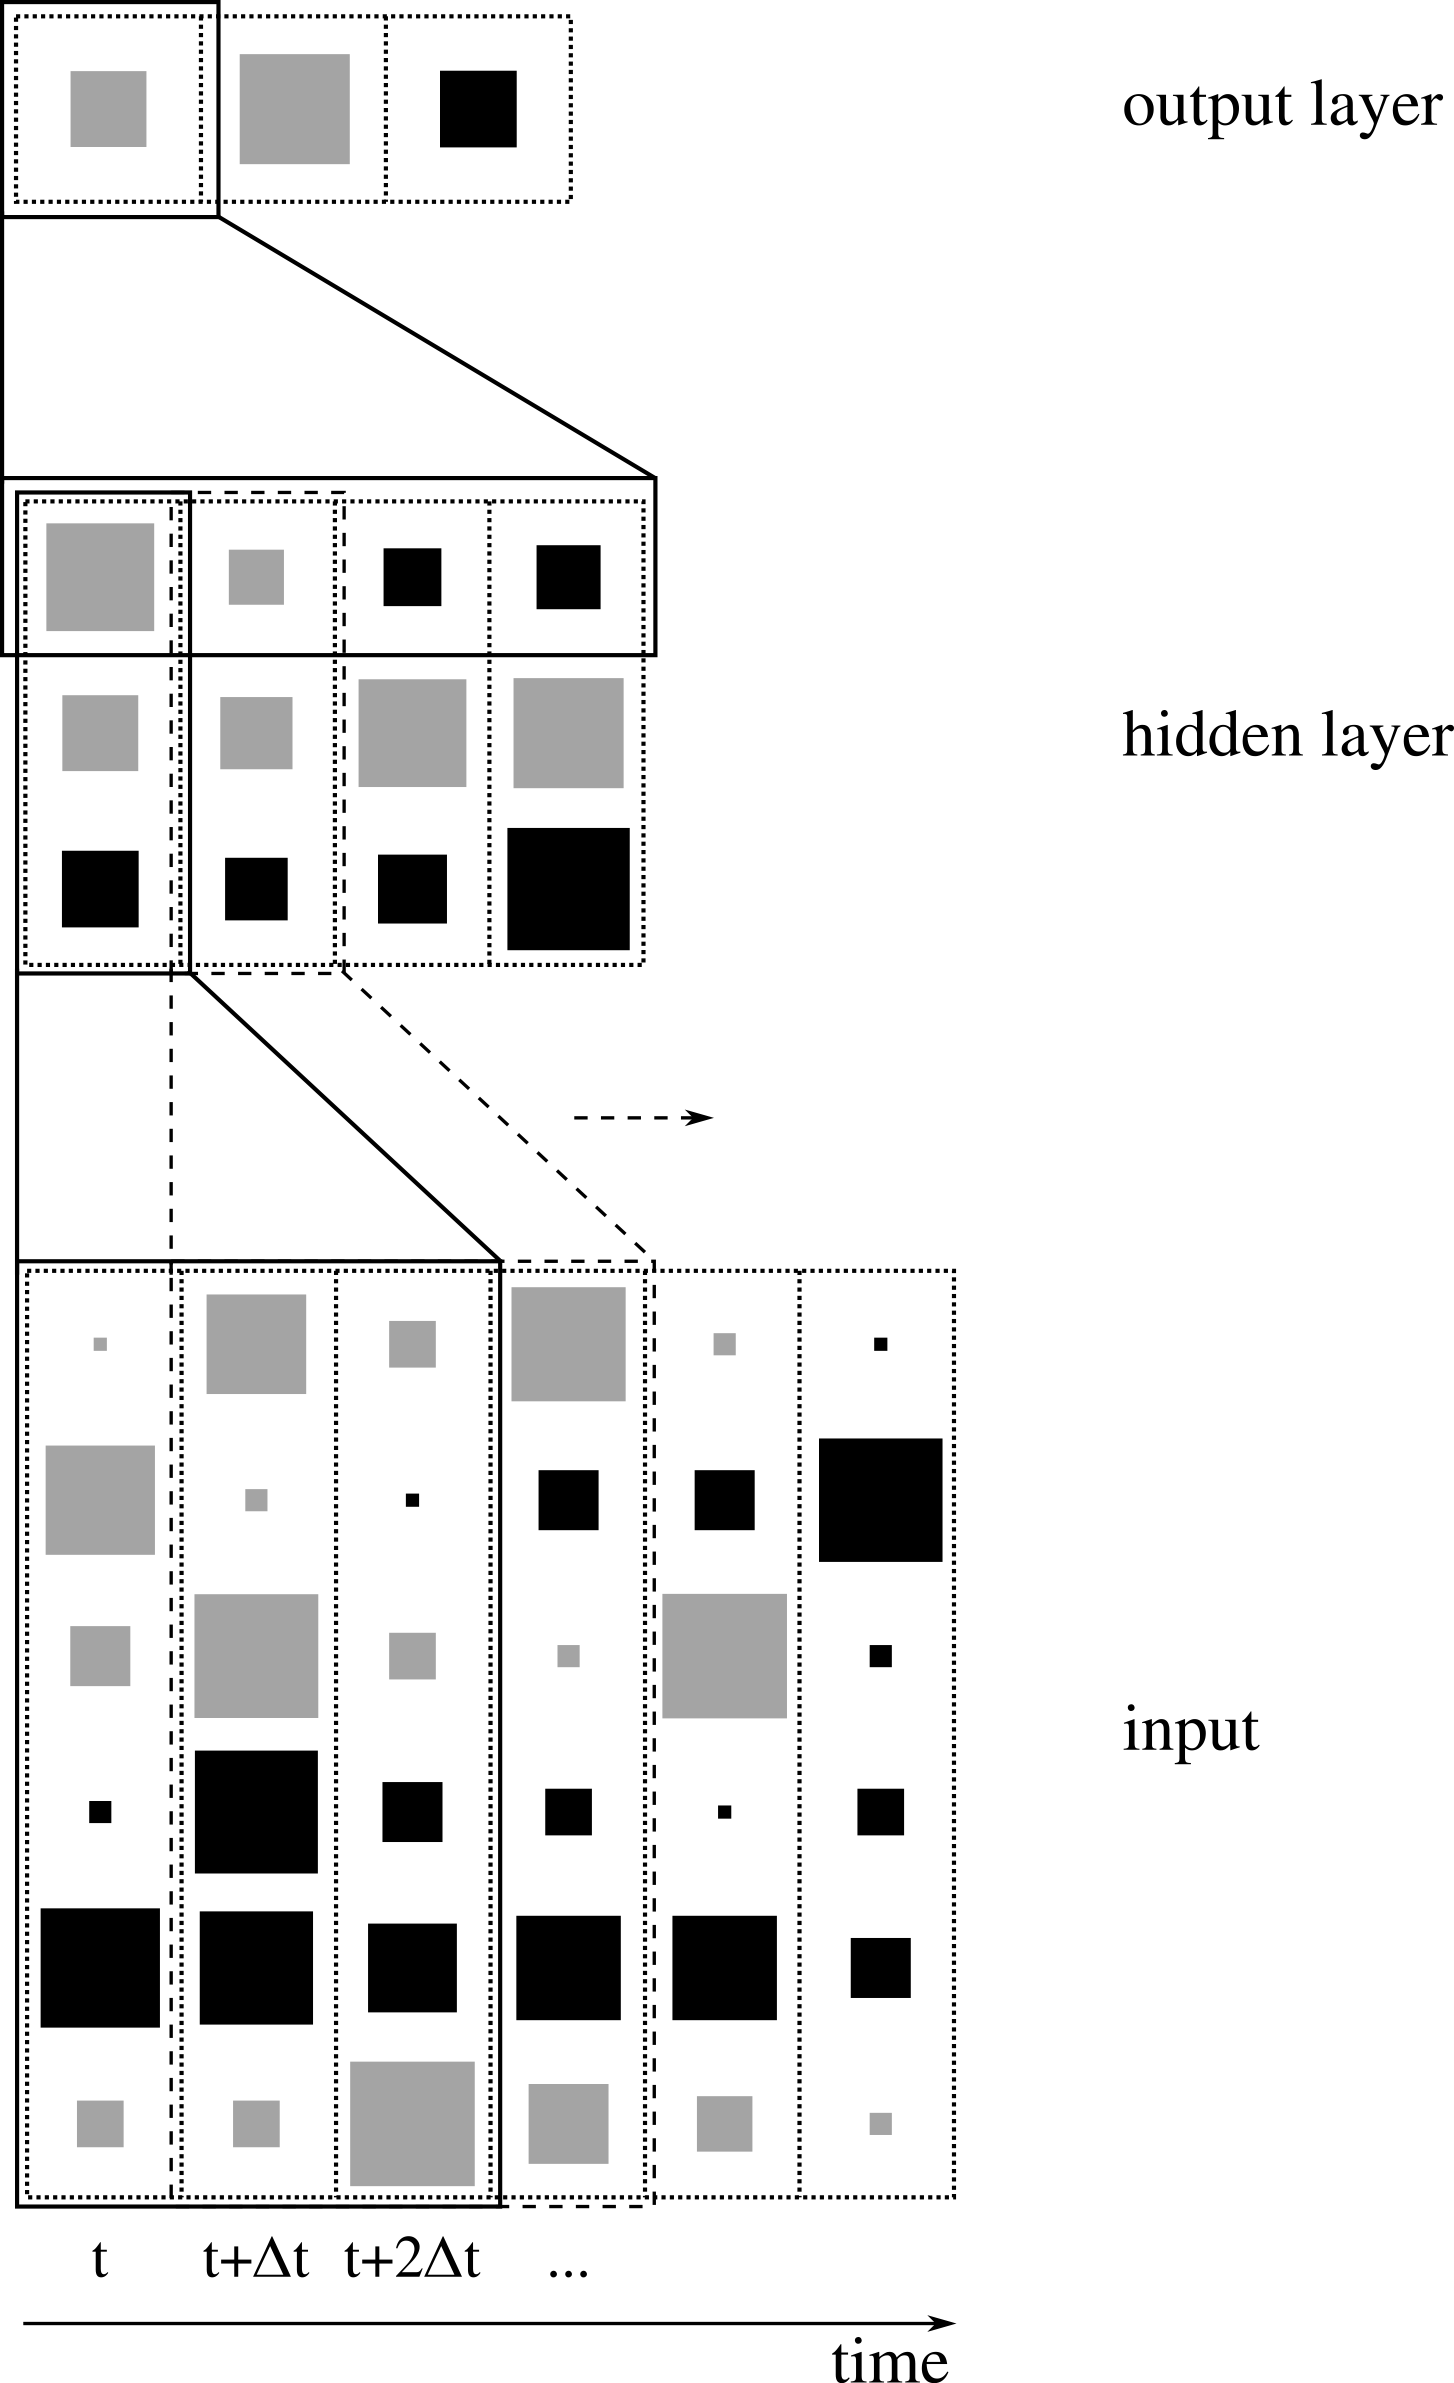
\includegraphics[width=0.3\paperwidth]{img/tdnn.png}}
		\caption{TDNN diagram \cite{WikipediaTDNN}.}
	\end{figure}
\end{center}

